% Options for packages loaded elsewhere
\PassOptionsToPackage{unicode}{hyperref}
\PassOptionsToPackage{hyphens}{url}
%
\documentclass[
]{article}
\usepackage{lmodern}
\usepackage{amssymb,amsmath}
\usepackage{ifxetex,ifluatex}
\ifnum 0\ifxetex 1\fi\ifluatex 1\fi=0 % if pdftex
  \usepackage[T1]{fontenc}
  \usepackage[utf8]{inputenc}
  \usepackage{textcomp} % provide euro and other symbols
\else % if luatex or xetex
  \usepackage{unicode-math}
  \defaultfontfeatures{Scale=MatchLowercase}
  \defaultfontfeatures[\rmfamily]{Ligatures=TeX,Scale=1}
\fi
% Use upquote if available, for straight quotes in verbatim environments
\IfFileExists{upquote.sty}{\usepackage{upquote}}{}
\IfFileExists{microtype.sty}{% use microtype if available
  \usepackage[]{microtype}
  \UseMicrotypeSet[protrusion]{basicmath} % disable protrusion for tt fonts
}{}
\makeatletter
\@ifundefined{KOMAClassName}{% if non-KOMA class
  \IfFileExists{parskip.sty}{%
    \usepackage{parskip}
  }{% else
    \setlength{\parindent}{0pt}
    \setlength{\parskip}{6pt plus 2pt minus 1pt}}
}{% if KOMA class
  \KOMAoptions{parskip=half}}
\makeatother
\usepackage{xcolor}
\IfFileExists{xurl.sty}{\usepackage{xurl}}{} % add URL line breaks if available
\IfFileExists{bookmark.sty}{\usepackage{bookmark}}{\usepackage{hyperref}}
\hypersetup{
  pdftitle={Documentación de texto},
  pdfauthor={Marcelo Bussetti},
  hidelinks,
  pdfcreator={LaTeX via pandoc}}
\urlstyle{same} % disable monospaced font for URLs
\usepackage[margin=1in]{geometry}
\usepackage{longtable,booktabs}
% Correct order of tables after \paragraph or \subparagraph
\usepackage{etoolbox}
\makeatletter
\patchcmd\longtable{\par}{\if@noskipsec\mbox{}\fi\par}{}{}
\makeatother
% Allow footnotes in longtable head/foot
\IfFileExists{footnotehyper.sty}{\usepackage{footnotehyper}}{\usepackage{footnote}}
\makesavenoteenv{longtable}
\usepackage{graphicx,grffile}
\makeatletter
\def\maxwidth{\ifdim\Gin@nat@width>\linewidth\linewidth\else\Gin@nat@width\fi}
\def\maxheight{\ifdim\Gin@nat@height>\textheight\textheight\else\Gin@nat@height\fi}
\makeatother
% Scale images if necessary, so that they will not overflow the page
% margins by default, and it is still possible to overwrite the defaults
% using explicit options in \includegraphics[width, height, ...]{}
\setkeys{Gin}{width=\maxwidth,height=\maxheight,keepaspectratio}
% Set default figure placement to htbp
\makeatletter
\def\fps@figure{htbp}
\makeatother
\usepackage[normalem]{ulem}
% Avoid problems with \sout in headers with hyperref
\pdfstringdefDisableCommands{\renewcommand{\sout}{}}
\setlength{\emergencystretch}{3em} % prevent overfull lines
\providecommand{\tightlist}{%
  \setlength{\itemsep}{0pt}\setlength{\parskip}{0pt}}
\setcounter{secnumdepth}{-\maxdimen} % remove section numbering

\title{Documentación de texto}
\author{Marcelo Bussetti}
\date{10/10/2020}

\begin{document}
\maketitle

\hypertarget{tuxedtulo-1}{%
\section{Título 1}\label{tuxedtulo-1}}

\hypertarget{tuxedtulo-2}{%
\subsection{Título 2}\label{tuxedtulo-2}}

\hypertarget{tuxedtulo-3}{%
\subsubsection{Título 3}\label{tuxedtulo-3}}

a

Título 6

El texto se ecribe en forma regular, puede incluir código de \texttt{R}
o expresiones en \(\LaTeX\)

Una nueva línea necesita doble enter!

Para sumar texto en \emph{cursiva} podemos usar el asterísco \emph{así
como ahora} o bien el guión bajo \emph{de esta forma}

Para sumar texto en \textbf{negrita} podemos usar el doble asterísco
\textbf{así como ahora} o bien el doble guión bajo \textbf{de esta
forma}

Los superíndices se declaran con el \textbf{\emph{sombrerito}} de la
siguiente manera: super\textsuperscript{3}

El código ASCII de la \emph{olita \textasciitilde{}} es ALT 126 y
Markdown la usa para \sout{tachar una frase}

declarar un link: \href{http://www.4ns.com.ar}{link}

Guión corto: -- es así.

Gión largo: --- de esta manera.

Ecuaciones en línea: \(S = \pi\cdot r^2\)

incorporar una imagen 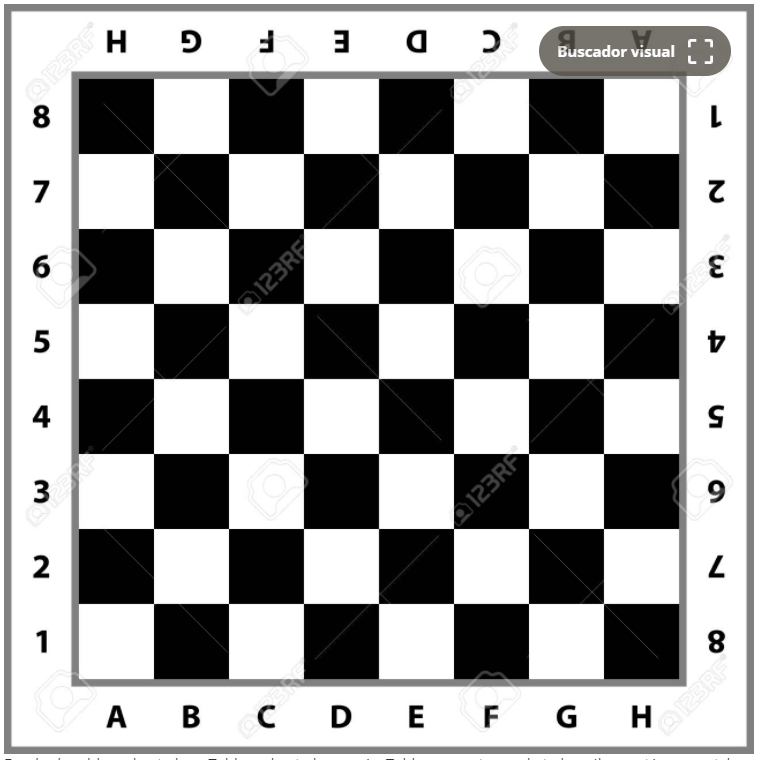
\includegraphics{tableroajedres.png}

\begin{center}\rule{0.5\linewidth}{0.5pt}\end{center}

una linea divisoria!

\hypertarget{listas-no-ordenadas}{%
\paragraph{Listas no ordenadas}\label{listas-no-ordenadas}}

\begin{itemize}
\tightlist
\item
  a
\item
  b
\item
  c

  \begin{itemize}
  \tightlist
  \item
    c1
  \item
    c2

    \begin{itemize}
    \tightlist
    \item
      c2a
    \end{itemize}
  \end{itemize}
\end{itemize}

\hypertarget{listas-ordenadas}{%
\paragraph{Listas ordenadas}\label{listas-ordenadas}}

\begin{enumerate}
\def\labelenumi{\arabic{enumi}.}
\tightlist
\item
  a
\item
  b
\item
  c

  \begin{enumerate}
  \def\labelenumii{\arabic{enumii}.}
  \tightlist
  \item
    c1
  \item
    c2

    \begin{enumerate}
    \def\labelenumiii{\arabic{enumiii}.}
    \tightlist
    \item
      c2a
    \end{enumerate}
  \end{enumerate}
\end{enumerate}

\hypertarget{tablas}{%
\subsubsection{Tablas}\label{tablas}}

\begin{longtable}[]{@{}lll@{}}
\toprule
alumno & edad & nota\tabularnewline
\midrule
\endhead
marcelo & 45 & 9\tabularnewline
\bottomrule
\end{longtable}

\end{document}
